\documentclass[UTF8]{ctexart}
\ctexset { section = { format={\Large \bfseries } } }
\pagestyle{plain}
\usepackage{float}
\usepackage{amsmath}
\usepackage{amssymb}
\usepackage{listings}
\usepackage{graphicx}%插入图片宏包
\usepackage{xcolor}
\usepackage{geometry}
\geometry{a4paper,scale=0.8}
\usepackage{caption}
\usepackage{subcaption}
\captionsetup[figure]{name={Figure}}
\captionsetup[table]{name={Table}}


\lstset{
language=Python, % 设置语言
basicstyle=\ttfamily, % 设置字体族
breaklines=true, % 自动换行
keywordstyle=\bfseries\color{blue}, % 设置关键字为粗体,
morekeywords={}, % 设置更多的关键字,用逗号分隔
emph={self}, % 指定强调词,如果有多个,用逗号隔开
emphstyle=\bfseries\color{Rhodamine}, % 强调词样式设置
commentstyle=\color{black!50!white}, % 设置注释样式,斜体,浅灰色
stringstyle=\bfseries\color{red!90!black}, % 设置字符串样式
columns=flexible,
numbers=left, % 显示行号在左边
numbersep=2em, % 设置行号的具体位置
numberstyle=\footnotesize, % 缩小行号
frame=single, % 边框
framesep=1em % 设置代码与边框的距离
}

\title{\textbf{Image Processing Homework 3}}
\author{吴嘉骜 21307130203}
\date{\today}

\begin{document}

\maketitle

\noindent
\section{}
\setlength{\parindent}{0pt}
Program the following based on spatial filters in the image domain:\\
(1) Smoothing operation.\\
(2) Sharpening algorithm.\\
Then, apply the algorithms to an image and display a comparison with the original image.\\
\textbf{Solution}:\\
(1) Smoothing operation.\\
The code is shown below:
\begin{lstlisting}
from PIL import Image
import numpy as np
import imgconvolution as ic

def smooth_box(img, size):
    """
    Smooths an image using a box filter of size size * size.
    
    Parameters:
        - img: the image to be smoothed, a 2D numpy array
        - size: the size of the box filter, an odd integer
        
    Returns:
        - img_smoothed: the smoothed image
    """
    kernel = np.ones((size, size)) / (size * size)
    img_smoothed = ic.convol(img, kernel)
    img_smoothed = np.clip(img_smoothed, 0, 255)

    return img_smoothed


def smooth_gauss(img, sigma):
    """
    Smooths an image using a Gaussian filter with standard deviation sigma.
    
    Parameters:
        - img: the image to be smoothed, a 2D numpy array
        - sigma: the standard deviation of the Gaussian filter
        
    Returns:
        - img_smoothed: the smoothed image
    """
    size = int(6 * sigma)
    if size % 2 == 0:  # Ensure the size is odd
        size += 1
    
    pad_size = size//2
    # generate Gaussian kernel.
    x = np.arange(-pad_size, pad_size + 1)
    ker = np.exp(-0.5 * (x / sigma) ** 2)
    ker = ker / np.sum(ker)
    ker = np.outer(ker, ker)
    img_smoothed = ic.convol(img, ker)
    img_smoothed = np.clip(img_smoothed, 0, 255)
    
    return img_smoothed

def smooth_medianorder(img, size):
    '''
    Smooths an image using a median filter.
    
    Parameters:
        - img: the image to be smoothed, a 2D numpy array
        - size: the size of the filter, an odd integer
        
    Returns:
        - img_smoothed: the smoothed image
    '''
    if size % 2 == 0:
        raise ValueError("size must be an odd integer")
    
    h, w = img.shape
    pad_size = size // 2
    img_padded = np.pad(img, pad_size, mode='edge')
    img_smoothed = np.zeros_like(img)
    
    for i in range(h):
        for j in range(w):
            img_smoothed[i, j] = np.median(img_padded[i:i+size, j:j+size])
            
    return img_smoothed
\end{lstlisting}
\textbf{Code interpretation}:\\
This code implements three smoothing operations: box filter (linear average with equal weights), Gaussian filter and median filter.
The median filter is implemented by replacing each pixel with the median of its neighborhood.
The box filter and Gaussian filter are implemented by convolving the image with the corresponding kernel, and the covolution is implemented by the function \texttt{convol} in \texttt{imgconvolution.py}.
For convenience, we list its code here:
\begin{lstlisting}
    def convol(img, kernel):
    """
    Convolves a 2D image with a kernel.
    
    Parameters:
        - img: the image to be convolved, a 2D numpy array
        - kernel: the kernel to convolve the image with
        
    Returns:
        - the convolved image numpy array with float values and the same size as the input image
    """
    if img.ndim != 2:
        raise ValueError('The image must be a 2D numpy array.')
    h, w = img.shape
    
    # Ensure the kernel is 2D
    if kernel.ndim == 1:
        kernel = kernel.reshape((1, -1))

    k_h, k_w = kernel.shape
    convol_img = np.zeros((h, w))
    rot_k = np.rot90(np.rot90(kernel))  # rotate the kernel 180 degrees
    
    # pad the image with zeros
    pad_h = int((k_h - 1)/2)
    pad_w = int((k_w - 1)/2)
    pad_img = np.zeros((h + 2 * pad_h, w + 2 * pad_w))
    pad_img[pad_h:pad_h + h, pad_w:pad_w + w] = img
    
    # convolve the image
    for i in range(h):
        for j in range(w):
            value = np.sum(pad_img[i:i + k_h, j:j + k_w] * rot_k)
            if value > 255:
                value = 255
            elif value < 0:
                value = 0
            convol_img[i,j] = value
            
    return convol_img
\end{lstlisting}
We test the first two algorithms on a test pattern. The result is as follows:\\
\begin{figure}[htbp]
    \centering
    % 第一行三张图片
    \begin{subfigure}{0.3\textwidth}
        \centering
        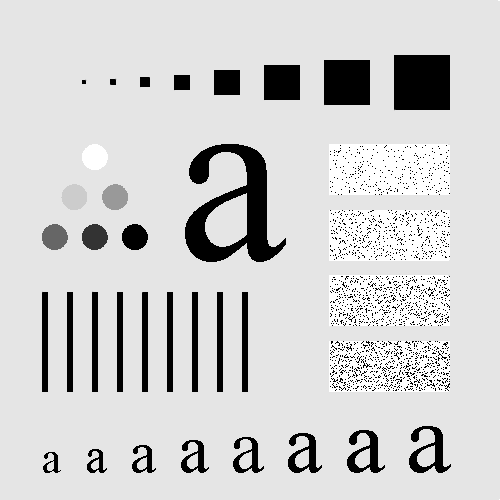
\includegraphics[width=\linewidth]{test_pattern_blurring.png}
        \caption{Input original image}
    \end{subfigure}%
    \hfill
    \begin{subfigure}{0.3\textwidth}
        \centering
        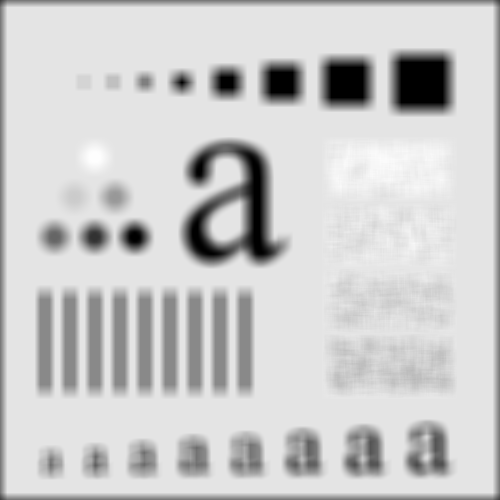
\includegraphics[width=\linewidth]{pattern_box_smooth.png}
        \caption{Box kernel, $15\times15$}
    \end{subfigure}%
    \hfill
    \begin{subfigure}{0.3\textwidth}
        \centering
        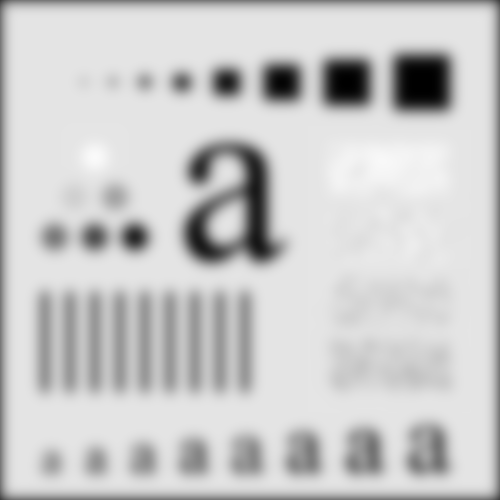
\includegraphics[width=\linewidth]{pattern_gauss_smooth.png}
        \caption{Gaussian kernel, $43\times43, \sigma = 7$}
    \end{subfigure}

    \caption{Image after smoothing}
\end{figure}

We can see that the original image is blurred and the edges are smoothed after smoothing.\\

Then, we test the median filter on a noisy image, together with Guassian kernel for comparison. The result is as follows:\\
\begin{figure}[htbp]
    \centering
    % 第一行三张图片
    \begin{subfigure}{0.3\textwidth}
        \centering
        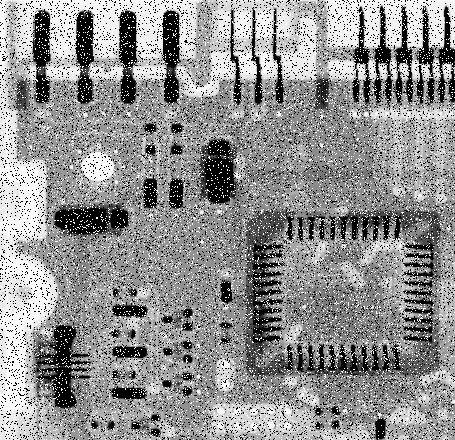
\includegraphics[width=\linewidth]{ckt_board.png}
        \caption{Input original image}
    \end{subfigure}%
    \hfill
    \begin{subfigure}{0.3\textwidth}
        \centering
        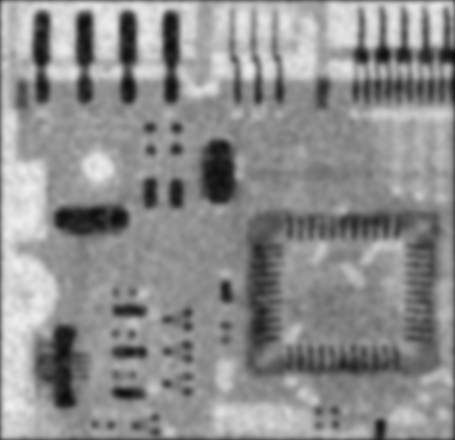
\includegraphics[width=\linewidth]{ckt_gauss_smooth.png}
        \caption{Gaussian kernel, $19\times19,\sigma = 3$}
    \end{subfigure}%
    \hfill
    \begin{subfigure}{0.3\textwidth}
        \centering
        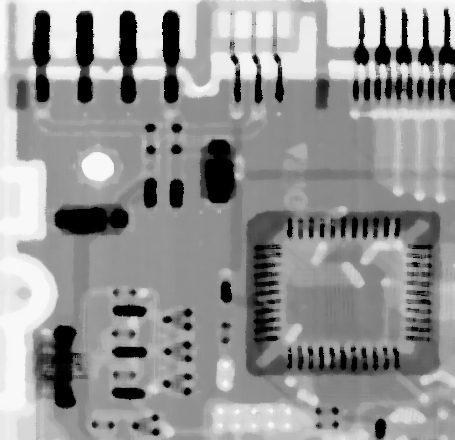
\includegraphics[width=\linewidth]{ckt_median_smooth.png}
        \caption{Median filter smooth, $7\times7$}
    \end{subfigure}

    \caption{Noise reduction by smoothing}
\end{figure}
\newpage
We can see that the Gaussian kernel smooths the image but does not remove the noise, while the median filter removes the noise effectively.\\
(2) Sharpening algorithm.\\
The code is shown below:
\begin{lstlisting}
from PIL import Image
import numpy as np
import imgconvolution as ic

def sharpen_laplace(img):
    '''
    Sharpens an image using the Laplace operator.
    
    Parameters:
        - img: the image to be sharpened, a 2D numpy array
        
    Returns:
        - img_sharpened: the sharpened image
    '''
    kernel = np.array([[1, 1, 1], [1, -8, 1], [1, 1, 1]])
    laplace_img = ic.convol(img, kernel)
    img_sharpened = img - laplace_img
    img_sharpened = np.clip(img_sharpened, 0, 255)
    return img_sharpened


def sharpen_masking(img, factor):
    '''
    Sharpens an image using high-boost filtering.

    Parameters:
        - img: the image to be sharpened, a 2D numpy array
        - factor: the boost factor. A value of 1 means no boost.

    Returns:
        - img_sharpened: the sharpened image
    '''
    import smoothen
    
    blurred_img = smoothen.smooth_gauss(img, 5)
    mask = img - blurred_img
    img_sharpened = img + factor * mask
    img_sharpened = np.clip(img_sharpened, 0, 255)
    return img_sharpened
\end{lstlisting}
\textbf{Code interpretation}:\\
This code implements two sharpening algorithms: Laplace operator and high-boost filtering. For Laplacian kernel, we use the following kernel:
\[
\begin{bmatrix}
    1 & 1 & 1\\
    1 & -8 & 1\\
    1 & 1 & 1
\end{bmatrix}
\]
The high-boost filtering is implemented by subtracting a blurred image from the original image, and then adding the result to the original image with a factor.
For simplicity, we use Gaussian filter to blur the image.\\
We test the first algorithm on blurred moon image. The result is as follows:\\
\begin{figure}[htbp]
    \centering
    \begin{subfigure}{0.3\textwidth}
        \centering
        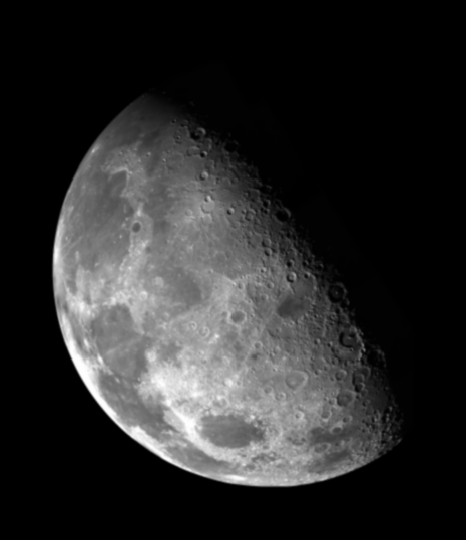
\includegraphics[width=\linewidth]{blurry_moon.png}
        \caption{Input original image}
    \end{subfigure}%
    \hspace{0.1\textwidth} % 调整这里的距离
    \begin{subfigure}{0.3\textwidth}
        \centering
        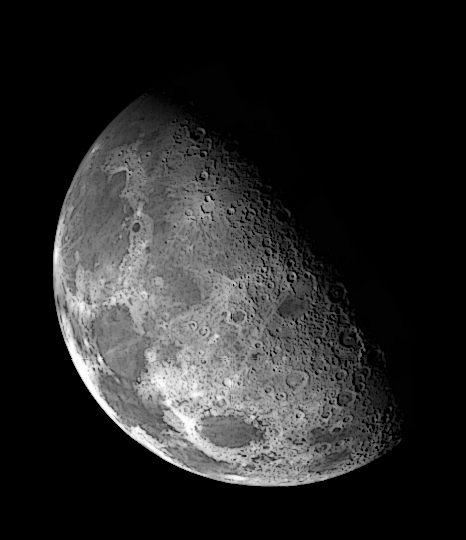
\includegraphics[width=\linewidth]{moon_laplace_sharpen.png}
        \caption{Laplacian kernel}
    \end{subfigure}

    \caption{Image after Laplace sharpening}
\end{figure}

We notice a significant improvement in sharpness using Laplace operator.\\

Then, we test the two algorithms on a slightly blurred image of white text on a dark gray background. The result is as follows:\\
\begin{figure}[htbp]
    \centering
    % 第一行三张图片
    \begin{subfigure}{0.3\textwidth}
        \centering
        
\includegraphics[width=\linewidth]{dipxe_text.png}
        \caption{Input original image}
    \end{subfigure}%
    \hfill
    \begin{subfigure}{0.3\textwidth}
        \centering
        
\includegraphics[width=\linewidth]{dipxe_text_laplace_sharpen.png}
        \caption{Laplacian kernel}
    \end{subfigure}%
    \hfill
    \begin{subfigure}{0.3\textwidth}
        \centering
        
\includegraphics[width=\linewidth]{dipxe_text_masking_sharpen.png}
        \caption{Unsharp masking, $k=1$}
    \end{subfigure}
    \hfill
    \begin{subfigure}{0.3\textwidth}
        \centering
        
\includegraphics[width=\linewidth]{dipxe_text_highboost_sharpen.png}
        \caption{Highboost filtering, $k=4.5$}
    \end{subfigure}

    \caption{Unsharp masking and highboost filtering}
\end{figure}

As we can see, this image is sharper than the original image by using Laplacian kernel, but with unsharp masking the effect will be more
significant. The highboost filtering gives more black halos around the border of the characters than unsharp masking, but the characters are
sharper than unsharp masking.\\


\section{}
Prove the following:\\
(1) Prove that the Fourier transform of an impulse train is also an impulse train.\\
(2) Prove that the discrete frequency domain transform of a real signal $f(x)$ is conjugate symmetric.\\
(3) Prove the convolution theorem for the discrete frequency domain/Fourier transform of a two-dimensional variable.\\
\textbf{Proof}:\\
(1)\\
An impulse train can be represented as:
\[
s_{\Delta T} (t) = \sum_{n=-\infty}^{\infty} \delta(t - n\Delta T)
\]
where \( \delta(t) \) is the Dirac delta function, and \( \Delta T \) is the spacing between the impulses.\\
The impulse train is periodic with a period of \( T = \Delta T \), so it can also be represented as a Fourier series:
\[
s_{\Delta T} (t) = \sum_{k=-\infty}^{\infty} c_k e^{j2\pi \frac{k}{\Delta T} t}
\]
where \( c_k \) is the Fourier coefficient.\\
The Fourier coefficient is given by:
\begin{equation*}
    \begin{aligned}
        c_k &= \frac{1}{\Delta T} \int_{-\frac{\Delta T}{2}}^{\frac{\Delta T}{2}} s_{\Delta T} (t) e^{-j2\pi \frac{k}{\Delta T} t} \, dt
        &= \frac{1}{\Delta T} \int_{-\frac{\Delta T}{2}}^{\frac{\Delta T}{2}} \delta(t) e^{-j2\pi \frac{k}{\Delta T} t} \, dt
        &= \frac{1}{\Delta T} \int_{-\infty}^{\infty} \delta(t) e^{-j2\pi \frac{k}{\Delta T} t} \, dt\\
        &= \frac{1}{\Delta T} e^0 = \frac{1}{\Delta T}
    \end{aligned}
\end{equation*}

The Fourier Transform of the impulse train is:
\[
S(u) = \mathcal{F}\{s_{\Delta T} (t)\} = \mathcal{F} \left\{ \sum_{k=-\infty}^{\infty} \frac{1}{\Delta T} e^{j2\pi \frac{k}{\Delta T} t} \right\} 
= \frac{1}{\Delta T} \sum_{k=-\infty}^{\infty} \mathcal{F}\{e^{j2\pi \frac{k}{\Delta T} t}\}
= \frac{1}{\Delta T} \sum_{k=-\infty}^{\infty} \delta \left( u - \frac{k}{\Delta T} \right)
\]
The last step is because the Fourier Transform of $\delta(t-t_0)$ is $e^{-j2\pi ut_0}$, and then the Fourier Transform of
$e^{-j2\pi tt_0}$ is $\delta(-u-t_0) = \delta(u+t_0)$. Subsitute $t_0 = -\frac{k}{\Delta T}$, we know that the Fourier Transform of
\( e^{j2\pi \frac{k}{\Delta T} t} \) is \( \delta \left( u - \frac{k}{\Delta T} \right) \).\\
From the result above, we notice that this is an impulse train in the frequency domain with a period of \( f = \frac{1}{\Delta T} \). 
Thus, the Fourier Transform of an impulse train is also an impulse train.\\
(2)\\
For a real signal \( f(x) \), its Discrete Fourier Transform (DFT) is defined as:
\[
F(u) = \sum_{x=0}^{M-1} f(x) e^{-j2\pi \frac{ux}{M}}
\]

To prove conjugate symmetry, consider the complex conjugate of \( F(u) \):
\[
\begin{aligned}
F^*(u) &= \left( \sum_{x=0}^{M-1} f(x) e^{-j2\pi \frac{ux}{M}} \right)^* \\
&= \sum_{x=0}^{M-1} f^*(x) e^{j2\pi \frac{ux}{M}} \\
&= \sum_{x=0}^{M-1} f(x) e^{-j2\pi \frac{-ux}{M}} \\
&= F(-u)
\end{aligned}
\]
where the second step is because \( f(x) \) is a real signal, so \( f^*(x) = f(x) \).\\
Thus, \( F(u) \) is conjugate symmetric.\\
(3)\\
For a 2-D signal $f(x,y)$, its Discrete Fourier Transform (DFT) is defined as:
\begin{equation}
    \begin{aligned}
        F(u, v) &= \sum_{x=0}^{M-1} \sum_{y=0}^{N-1} f(x, y) e^{-j2\pi \left( \frac{ux}{M} + \frac{vy}{N} \right)} \\
    \end{aligned}
\end{equation}
And the Inverse Discrete Fourier Transform (IDFT) is defined as:
\begin{equation}
    \begin{aligned}
        f(x, y) &= \frac{1}{MN} \sum_{u=0}^{M-1} \sum_{v=0}^{N-1} F(u, v) e^{j2\pi \left( \frac{ux}{M} + \frac{vy}{N} \right)} \\
    \end{aligned}
\end{equation}

For two-dimensional signals \( f(x, y) \) and \( h(x, y) \), their discrete convolution is defined as:
\begin{equation}
    (f * h)(x, y) = \sum_{m=0}^{M-1} \sum_{n=0}^{N-1} f(m, n) h(x-m, y-n)
\end{equation}
Our goal is to prove that:\\
\begin{equation}
    (f * h)(x, y) \Leftrightarrow  (F \cdot H)(u, v)
\end{equation}
\begin{equation}
    (f \cdot h)(x, y) \Leftrightarrow \frac{1}{MN}(F * H)(u, v)
\end{equation}
where $F,H$ are the DFT of $f,h$ respectively, and the double arrow is used to indicate that the left and right sides of the expressions constitute a Fourier transform pair.\\
Suppose we have proved that a forward DFT $\mathcal{F}\{f(x,y)\}$ is $F(u,v)$ (the "$\Rightarrow$" part), then we can simply subsitute into equation (2) and then (1) to get
$\mathcal{F}^{-1}\{F(u,v)\} = f(x,y)$ (the "$\Leftarrow$" part). Details are explained in the following proof.\\
\begin{equation*}
    \begin{aligned}
    \mathcal{F}^{-1}\{F(u,v)\} &= \frac{1}{MN} \sum_{u=0}^{M-1} \sum_{v=0}^{N-1} F(u, v) e^{j2\pi \left( \frac{ux}{M} + \frac{vy}{N} \right)} \\
    &= \frac{1}{MN} \sum_{u=0}^{M-1} \sum_{v=0}^{N-1} \left( \sum_{m=0}^{M-1} \sum_{n=0}^{N-1} f(m, n) e^{-j2\pi \left( \frac{um}{M} + \frac{vn}{N} \right)} \right) e^{j2\pi \left( \frac{ux}{M} + \frac{vy}{N} \right)} \\
    &= \frac{1}{MN} \sum_{m=0}^{M-1} \sum_{n=0}^{N-1} f(m, n) \sum_{u=0}^{M-1} \sum_{v=0}^{N-1} e^{-j2\pi \left( \frac{um}{M} + \frac{vn}{N} \right)} e^{j2\pi \left( \frac{ux}{M} + \frac{vy}{N} \right)} \\
    &= \frac{1}{MN} \sum_{m=0}^{M-1} \sum_{n=0}^{N-1} f(m, n) \sum_{u=0}^{M-1} e^{j2\pi \left( \frac{u(x-m)}{M}\right)} \sum_{v=0}^{N-1} e^{j2\pi \left( \frac{v(y-n)}{N} \right)} \\
    &= \frac{1}{MN} \sum_{m=0}^{M-1} \sum_{n=0}^{N-1} f(m, n) \cdot M \delta_{m,x} \cdot N \delta_{n,y} \\
    &= f(x,y)
    \end{aligned}
\end{equation*}
The last step from the orthogonality condition:\\
\begin{equation*}
    \begin{aligned}
        \sum_{u=0}^{M-1} e^{-j2\pi \frac{um}{M} } e^{j2\pi  \frac{ux}{M} } = M \delta_{m,x}
    \end{aligned}
\end{equation*}
where $\delta_{m,x}$ is the Kronecker delta.\\
Therefore, we just need to prove the "$\Rightarrow$" part of (4) and (5) respectively.
\subsection*{Part 1: Proof of \( (f * h)(x, y) \Leftrightarrow  (F \cdot H)(u, v) \)}

Define \( g(x, y) = (f * h)(x, y) \). The DFT of \( g(x, y) \) is:
\[
\begin{aligned}
G(u, v) &= \sum_{x=0}^{M-1} \sum_{y=0}^{N-1} g(x, y) e^{-j2\pi \left( \frac{ux}{M} + \frac{vy}{N} \right)} \\
&= \sum_{x=0}^{M-1} \sum_{y=0}^{N-1} \left( \sum_{m=0}^{M-1} \sum_{n=0}^{N-1} f(m, n) h(x-m, y-n) \right) e^{-j2\pi \left( \frac{ux}{M} + \frac{vy}{N} \right)} \\
&= \sum_{m=0}^{M-1} \sum_{n=0}^{N-1} f(m, n) \sum_{x=0}^{M-1} \sum_{y=0}^{N-1} h(x-m, y-n) e^{-j2\pi \left( \frac{ux}{M} + \frac{vy}{N} \right)}.
\end{aligned}
\]

Let \( x' = x - m \) and \( y' = y - n \), implying \( x = x' + m \) and \( y = y' + n \). Note that this change of variables does not change the limits of the summation since the signals are periodic. To specify, 
given $m, n$, $x'$ ranges from $-m$ to $M-1-m$ and $y'$ ranges from $-n$ to $N-1-n$.\\ Since $p(x,y) = h(x,y)e^{-j2\pi \left( \frac{ux}{M} + \frac{vy}{N} \right)}$ is periodic, $p(x',y') = p(x'+M,y'+N)$,
we can change the range to $M-m, M-m+1, \ldots, 0, \ldots, M-1-m$ and $N-n, \ldots, 0, \ldots, N-1-n$, which is the same as $0, \ldots, M-1$ and $0, \ldots, N-1$.\\
Then we have:
\[
\begin{aligned}
    G(u, v) &= \sum_{m=0}^{M-1} \sum_{n=0}^{N-1} f(m, n) \sum_{x'=-m}^{M-1-m} \sum_{y'=-n}^{N-1-n} h(x', y') e^{-j2\pi \left( \frac{u(x'+m)}{M} + \frac{v(y'+n)}{N} \right)} \\
    &= \sum_{m=0}^{M-1} \sum_{n=0}^{N-1} f(m, n) e^{-j2\pi \left( \frac{um}{M} + \frac{vn}{N} \right)} \sum_{x'=-m}^{M-1-m} \sum_{y'=-n}^{N-1-n} h(x', y') e^{-j2\pi \left( \frac{ux'}{M} + \frac{vy'}{N} \right)} \\
    &= \sum_{m=0}^{M-1} \sum_{n=0}^{N-1} f(m, n) e^{-j2\pi \left( \frac{um}{M} + \frac{vn}{N} \right)} \sum_{x'=0}^{M-1} \sum_{y'=0}^{N-1} h(x', y') e^{-j2\pi \left( \frac{ux'}{M} + \frac{vy'}{N} \right)} \\
    &= \left( \sum_{m=0}^{M-1} \sum_{n=0}^{N-1} f(m, n) e^{-j2\pi \left( \frac{um}{M} + \frac{vn}{N} \right)} \right) \left( \sum_{x=0}^{M-1} \sum_{y=0}^{N-1} h(x, y) e^{-j2\pi \left( \frac{ux}{M} + \frac{vy}{N} \right)} \right) \\
    &= F(u, v) \cdot H(u, v).
\end{aligned}
\]
This completes the proof of the forward Fourier Transform for (4), and the inverse Fourier Transform holds as explained before.

\subsection*{Part 2: Proof of \( (f \cdot h)(x, y) \Leftrightarrow \frac{1}{MN}(F * H)(u, v) \)}

Denote $z(x,y) = (f \cdot h)(x, y)$, and $Z(u,v) = \mathcal{F}\{z(x,y)\}$.\\
We start by taking the DFT of the product of two signals \( f(x, y) \) and \( h(x, y) \).

\begin{equation*}
\begin{aligned}
Z(u,v) &= \sum_{x=0}^{M-1} \sum_{y=0}^{N-1} f(x, y) h(x, y) e^{-j2\pi \left( \frac{ux}{M} + \frac{vy}{N} \right)} \\
\end{aligned}
\end{equation*}
Then express \( f(x, y) \) and \( h(x, y) \) in terms of their inverse DFTs.

\begin{equation*}
\begin{aligned}
Z(u,v) &= \sum_{x=0}^{M-1} \sum_{y=0}^{N-1} \left( \frac{1}{MN} \sum_{u'=0}^{M-1} \sum_{v'=0}^{N-1} F(u', v') e^{j2\pi \left( \frac{u'x}{M} + \frac{v'y}{N} \right)} \right) \\
& \quad \cdot \left( \frac{1}{MN} \sum_{u''=0}^{M-1} \sum_{v''=0}^{N-1} H(u'', v'') e^{j2\pi \left( \frac{u''x}{M} + \frac{v''y}{N} \right)} \right) e^{-j2\pi \left( \frac{ux}{M} + \frac{vy}{N} \right)} \\
\end{aligned}
\end{equation*}

Now, we combine the exponential terms and rearrange the summations.

\begin{equation*}
\begin{aligned}
Z(u,v) &= \frac{1}{M^2 N^2} \sum_{u'=0}^{M-1} \sum_{v'=0}^{N-1} \sum_{u''=0}^{M-1} \sum_{v''=0}^{N-1} F(u', v') H(u'', v'') \\
& \quad \cdot \sum_{x=0}^{M-1} \sum_{y=0}^{N-1} e^{j2\pi \left( \frac{(u' + u'' - u)x}{M} + \frac{(v' + v'' - v)y}{N} \right)} \\
\end{aligned}
\end{equation*}

The inner double summation over \( x \) and \( y \) is a 2-D Dirichlet kernel, which evaluates to \( MN \) when \( u' + u'' = u \) and \( v' + v'' = v \) hold, and evaluates to 0 otherwise.
Thus, we have
\begin{equation*}
\begin{aligned}
Z(u,v) &= \frac{1}{MN} \sum_{u'=0}^{M-1} \sum_{v'=0}^{N-1} F(u', v') H(u - u', v - v') \\
&= \frac{1}{MN} (F * H)(u, v)
\end{aligned}
\end{equation*}
The final result shows that the DFT of the product of two signals is equal to the scaled convolution of their DFTs, completing the foward proof for the second part of the theorem.
The inverse proof holds as explained before.\\
In conclusion, we have proved the convolution theorem for the Fourier transform of a two-dimensional variable.

\end{document}